\documentclass{article}%book,report,letter

\usepackage{ctex}
\usepackage{fontspec}
%\usepackage{color}
%\usepackage{graphicx} %use graph format
%\usepackage{subfigure}
%\usepackage{epstopdf} %eps图片
\usepackage{amsmath}  %字体加粗
%\usepackage{math}
\usepackage{amsthm}
\usepackage{amssymb} %因为所以符号
%\usepackage{caption}
%\captionsetup[table]{labelsep=space}
\usepackage{float}%图片位置

%自定义命令
\newcommand*{\myTestTimes}{1\xspace}
%\typein[\myTestTimes]{这是第几次测试?}
\newcommand*{\myName}{桑明达\xspace}
\newcommand*{\myNumber}{15300180062\xspace}
\newcommand*{\myHomeworkNumber}{第十五周作业\xspace}
\newcommand*{\myArticleName}{微分方程数值解法\xspace}

\newcommand*{\myseries}[2][n]{\ensuremath{#2_1,#2_2,\dots,#2_{#1}}}


%制作页眉页脚
\usepackage{fancyhdr}
\pagestyle{fancy}
\lhead{\myHomeworkNumber}
\chead{\myArticleName}
\rhead{\myName \myNumber}
\lfoot{}
\cfoot{\thepage}
\rfoot{}
\renewcommand{\headrulewidth}{0.4pt}
\renewcommand{\footrulewidth}{0.4pt}

%标题
\title{\heiti \myArticleName \\ [2ex] \begin{large} \myHomeworkNumber \end{large}}
\author{\kaishu \myName \myNumber}
\date{\today}

% 正文区
\begin{document}
\maketitle
%\newpage


\section{P254 3 用线性有限元求解混合边值问题}

\begin{proof}

	我使用下面的$\mathbf{L}$、$\mathbf{F}$,计算结果如后图,偏差比较大,求正确求解方式

	$\mathbf{L}$=\begin{pmatrix}
	 a(\varphi _1,\varphi _1)&a(\varphi _1,\varphi _2)&  &  & \\
	 a(\varphi _2,\varphi _1)& a(\varphi _2,\varphi _2) & a(\varphi _2,\varphi _3) &  & \\
	 & a(\varphi _3,\varphi _2) & a(\varphi _3,\varphi _3) & \ddots & \\
	 &  & \ddots & \ddots & a(\varphi _{n-2},\varphi _{n-1}) \\
	 &  &  & a(\varphi _{n-1},\varphi _{n-2}) & a(\varphi _{n-1},\varphi _{n-1})+a(\varphi _{n-1},\varphi _{n})
	\end{pmatrix}

$\mathbf{F}$=\begin{pmatrix}
	 <f,\varphi _1>-u(0))a(\varphi _1,\varphi _0)\\
	 <f,\varphi _2>\\
	 <f,\varphi _3>\\
	 \vdots \\
	 <f,\varphi _{n-2}>\\
	 <f,\varphi _{n-1}>-hu'(1))a(\varphi _n,\varphi _{n-1})\\
	\end{pmatrix}



	\begin{figure}[H]
	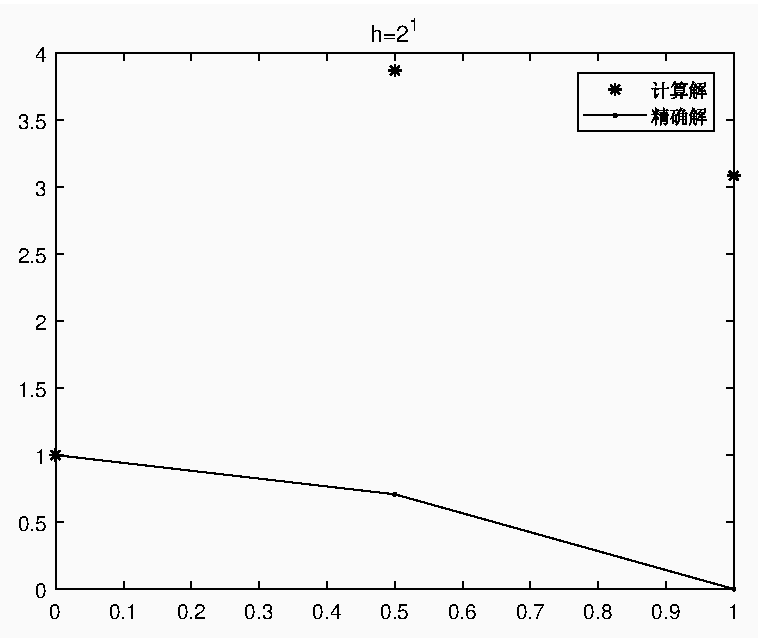
\includegraphics[width=1\linewidth]{week15_1_1.eps}
	\label{Fig:1}
	\end{figure}

	\begin{figure}[H]
	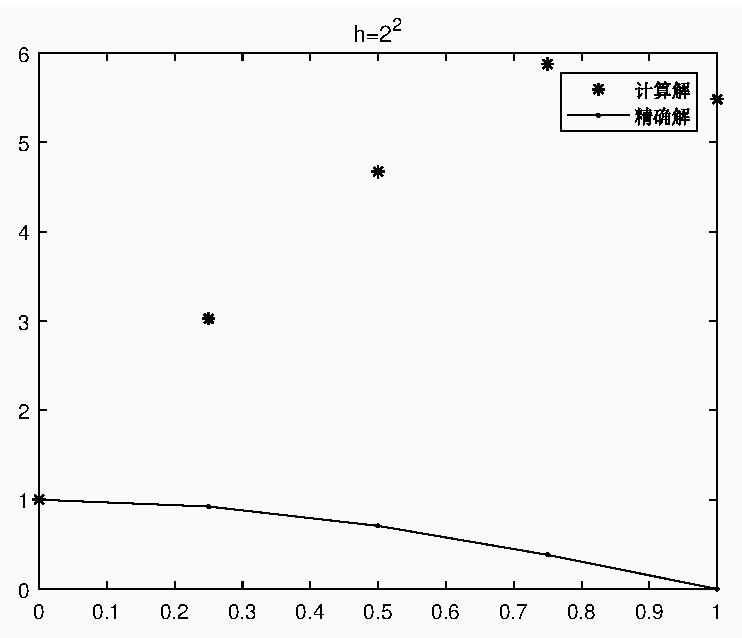
\includegraphics[width=1\linewidth]{week15_1_2.eps}
	\label{Fig:2}
	\end{figure}

	\begin{figure}[H]
	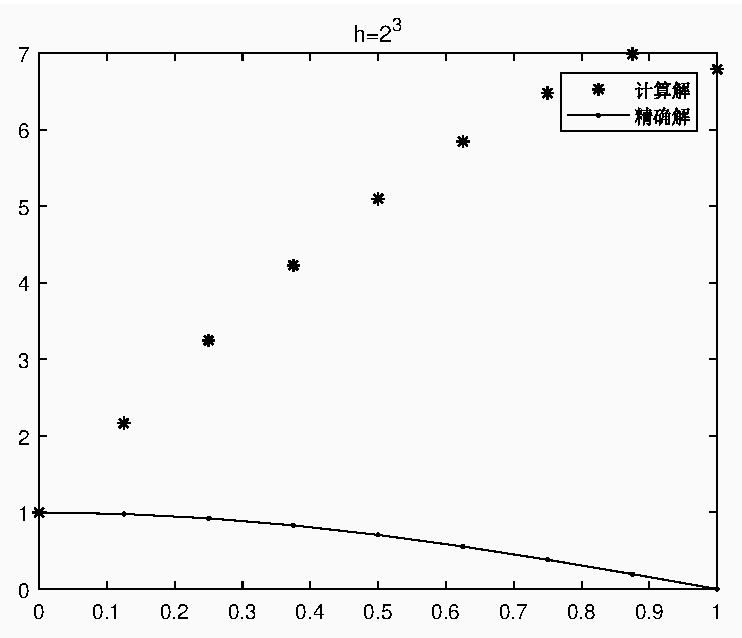
\includegraphics[width=1\linewidth]{week15_1_3.eps}
	\label{Fig:3}
	\end{figure}

	\begin{figure}[H]
	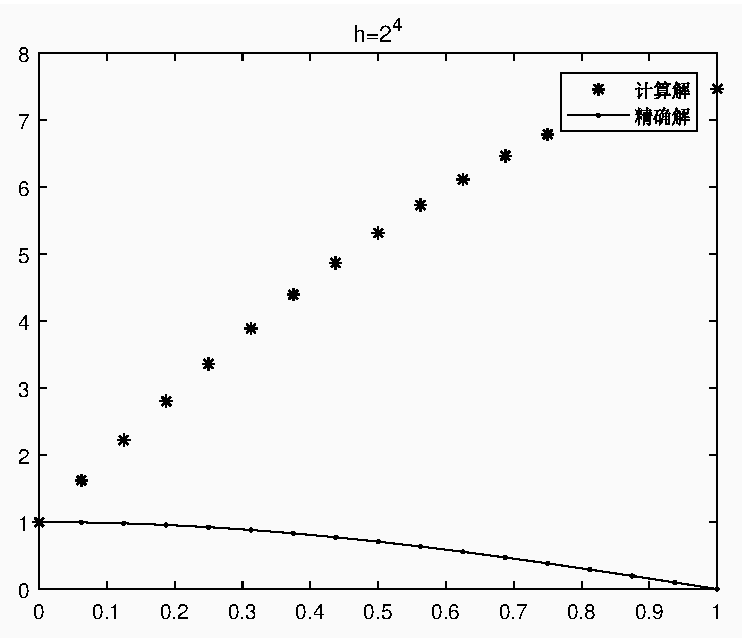
\includegraphics[width=1\linewidth]{week15_1_4.eps}
	\label{Fig:4}
	\end{figure}

	\begin{figure}[H]
	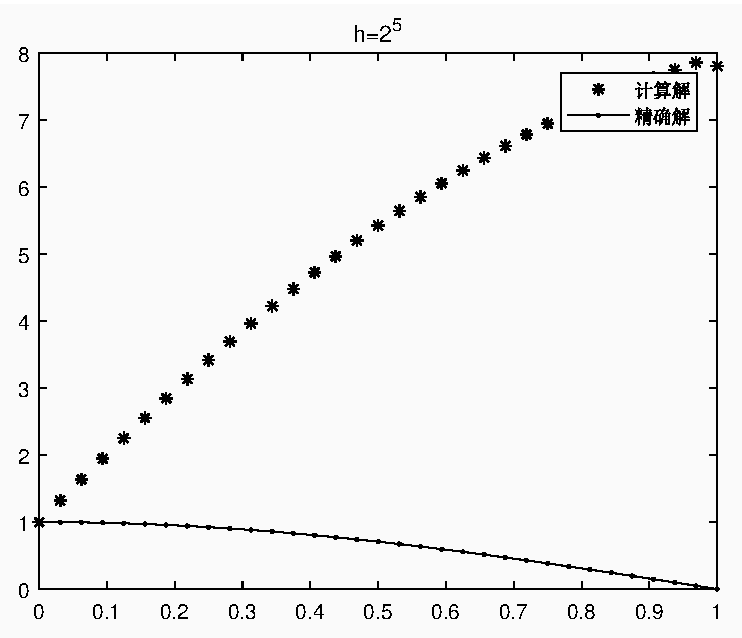
\includegraphics[width=1\linewidth]{week15_1_5.eps}
	\label{Fig:5}
	\end{figure}

	\begin{figure}[H]
	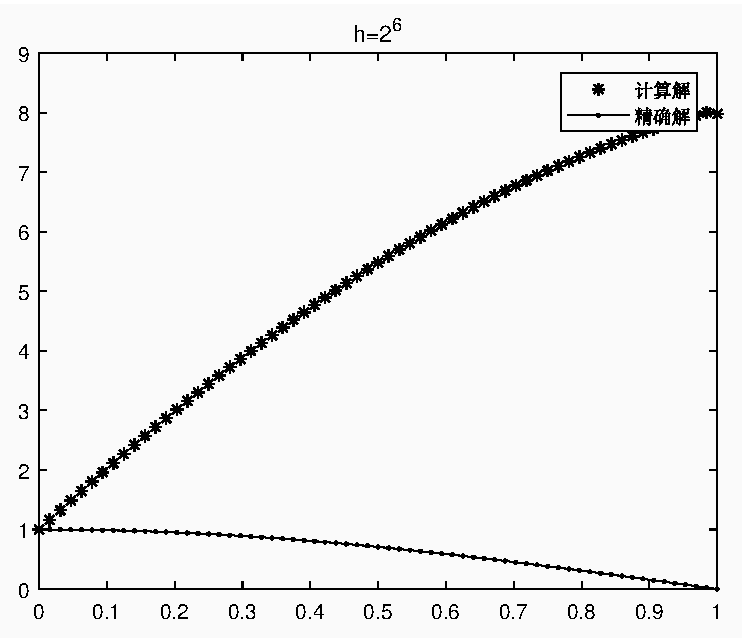
\includegraphics[width=1\linewidth]{week15_1_6.eps}
	\label{Fig:6}
	\end{figure}

\end{proof}


\end{document}
